
\iffalse
\chapter{2024}
\author{EE24BTECH11004}
\section{me}
\fi
%\begin{enumerate}

\item If '$\to$' denotes increasing order of intensity, then the meaning of the words 
$[$smile $\to$ giggle $\to$ laugh$]$ is analogous to $[$disapprove $\to$ \_\_\_\_\_\_ $\to$ chide$]$. 
Which one of the given options is appropriate to fill the blank?
\begin{enumerate}
    \item reprove
    \item praise
    \item reprise
    \item grieve
\end{enumerate}

\item Find the odd one out in the set: $\{19, 37, 21, 17, 23, 29, 31, 11\}$
\begin{enumerate}
    \item $21$
    \item $29$
    \item $37$
    \item $23$
\end{enumerate}
\item In the following series, identify the number that needs to be changed to form the Fibonacci series. 
\[
1, 1, 2, 3, 6, 8, 13, 21, \dots
\]
\begin{enumerate}
    \item $8$
    \item $21$
    \item $6$
    \item $13$
\end{enumerate}

\item The real variables $x$, $y$, $z$, and the real constants $p$, $q$, $r$ satisfy
\[
\frac{x}{pq - r^2} = \frac{y}{qr - p^2} = \frac{z}{rp - q^2}
\]
Given that the denominators are non-zero, the value of $px + qy + rz$ is
\begin{enumerate}
    \item $0$
    \item $1$
    \item $pqr$
    \item $p^2 + q^2 + r^2$
\end{enumerate}

\item Take two long dice (rectangular parallelepiped), each having four rectangular faces labeled as $2$, $3$, $5$, and $7$. If thrown, the long dice cannot land on the square faces and has $\frac{1}{4}$ probability of landing on any of the four rectangular faces. The label on the top face of the dice is the score of the throw.

If thrown together, what is the probability of getting the sum of the two long dice scores greater than $11$?
\begin{enumerate}
    \item $\frac{3}{8}$
    \item $\frac{1}{8}$
    \item $\frac{1}{16}$
    \item $\frac{3}{16}$
\end{enumerate}
\item In the given text, the blanks are numbered (i–iv) Select the best match for all the blanks.

Prof. P. (i) $\underline{\hspace{1cm}}$ merely a man who narrated funny stories. (ii) $\underline{\hspace{1cm}}$ in his blackest moments he was capable of self-deprecating humor.

Prof. Q. (iii) $\underline{\hspace{1cm}}$ a man who hardly narrated funny stories. (iv) $\underline{\hspace{1cm}}$ in his blackest moments was he able to find humor.
\begin{enumerate}
    \item (i) asn't \quad (ii) Only \quad (iii) Even \quad (iv) Even
    \item (i) was \quad (ii) Only \quad (iii) wasn't \quad (iv) Only
    \item (i) was \quad (ii) Even \quad (iii) wasn't \quad (iv) Only
    \item (i) wasn't \quad (ii) Only \quad (iii) was \quad (iv) Even
\end{enumerate}

\item How many combinations of non-null sets $A$, $B$, or $C$ are possible from the subsets of $\{ 2, 3, 5 \}$ satisfying the conditions: (i) $A$ is a subset of $B$, and (ii) $B$ is a subset of $C$?
\begin{enumerate}
    \item $28$
    \item $27$
    \item $18$
    \item $19$
\end{enumerate}

\item The bar chart gives the batting averages of $VK$ and $RS$ for 11 calendar years from 2012 to 2022. Considering that 2015 and 2019 are world cup years, which one of the following options is true?


\begin{tikzpicture}
    \begin{axis}[
        ybar=0pt,
        bar width=10pt,
        width=14cm, height=7cm,
        enlarge x limits=0.15,
        ymin=0, ymax=140,
        ylabel={Batting Average},
        xlabel={Calender Year},
        symbolic x coords={2012, 2013, 2014, 2015, 2016, 2017, 2018, 2019, 2020, 2021, 2022},
        xtick=data,
        legend pos=north west,
        ymajorgrids=true,
        grid style=dashed,
        nodes near coords,
        every node near coord/.append style={font=\tiny},
    ]
        % Data for VK
        \addplot[
            fill=gray!70,
            draw=black,
        ] coordinates {
            (2012,60) (2013,50) (2014,50) (2015,30) (2016,100) 
            (2017,60) (2018,140) (2019,60) (2020,50) (2021,20) (2022,40)
        };
        
        % Data for RS
        \addplot[
            pattern=north east lines,
            draw=black,
        ] coordinates {
            (2012,10) (2013,50) (2014,50) (2015,40) (2016,30) 
            (2017,70) (2018,80) (2019,60) (2020,60) (2021,40) (2022,50)
        };
        
        \legend{VK, RS}
    \end{axis}
\end{tikzpicture}


\begin{enumerate}
    \item $RS$ has a higher yearly batting average than that of $VK$ in every world cup year.
    \item $VK$ has a higher yearly batting average than that of $RS$ in every world cup year.
    \item $VK$'s yearly batting average is consistently higher than that of $RS$ between the two world cup years.
    \item $RS$'s yearly batting average is consistently higher than that of $VK$ in the last three years.
\end{enumerate}
\item A planar rectangular paper has two V-shaped pieces attached as shown below.
\begin{figure}[H]
\centering
\resizebox{0.5\textwidth}{!}{%
\begin{circuitikz}
\tikzstyle{every node}=[font=\normalsize]
\draw [short] (2.25,8.5) -- (6.75,8.5);
\draw [short] (6.75,8.5) -- (6.75,7.5);
\draw [short] (6.75,7.5) -- (2.25,7.5);
\draw [short] (2.25,8.5) -- (2.75,10);
\draw [short] (2.75,10) -- (3,10);
\draw [short] (3,10) -- (3.75,8.75);
\draw [short] (3.75,8.75) -- (4.25,8.75);
\draw [short] (4.25,8.75) -- (3.25,10.25);
\draw [short] (3.25,10.25) -- (2.5,10.25);
\draw [short] (2.5,10.25) -- (1.5,8.5);
\draw [short] (1.5,8.5) -- (1.5,7.25);
\draw [short] (2.25,7.5) -- (2.75,6.25);
\draw [short] (2.75,6.25) -- (3,6.25);
\draw [short] (3,6.25) -- (3.75,7.25);
\draw [short] (3.75,7.25) -- (4.25,7.25);
\draw [short] (4.25,7.25) -- (3.25,6);
\draw [short] (3.25,6) -- (2.5,6);
\draw [short] (2.5,6) -- (1.5,7.25);
\end{circuitikz}
}%

\end{figure}
This piece of paper is folded to make the following closed three-dimensional object.
 
 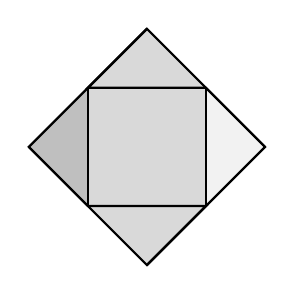
\begin{tikzpicture}[scale=1.5]

\coordinate (A) at (0,0);
\coordinate (B) at (1,1);
\coordinate (C) at (2,0);
\coordinate (D) at (1,-1);
\coordinate (E) at (0.5,-0.5);
\coordinate (F) at (1.5,-0.5);
\coordinate (G) at (0.5,0.5);
\coordinate (H) at (1.5,0.5);


\fill[gray!30] (A) -- (B) -- (H) -- (F) -- (D) -- cycle;


\fill[gray!50] (A) -- (E) -- (G) -- (B) -- cycle;

\fill[gray!10] (C) -- (H) -- (F) -- (D) -- cycle;

\draw[thick] (A) -- (B) -- (C) -- (D) -- cycle;
\draw[thick] (A) -- (E) -- (F) -- (D);
\draw[thick] (B) -- (G) -- (H) -- (C);
\draw[thick] (E) -- (G);
\draw[thick] (F) -- (H);

\end{tikzpicture}

The number of folds required to form the above object is:
\begin{enumerate}
        \item $9$
        \item $7$
        \item $11$
        \item $8$
    \end{enumerate}

    \item Four equilateral triangles are used to form a regular closed three-dimensional object by joining along the edges. The angle between any two faces is:
    \begin{enumerate}
        \item $30^\circ$
        \item $60^\circ$
        \item $45^\circ$
        \item $90^\circ$
    \end{enumerate}
 \item In order to numerically solve the ordinary differential equation $\frac{dy}{dt} = -y$ for $t > 0$, with an initial condition $y(0) = 1$, the following scheme is employed
    \[
    \frac{y_{n+1} - y_n}{\Delta t} = -\frac{1}{2} (y_{n+1} + y_n).
    \]
    Here, $\Delta t$ is the time step and $y_n = y(n\Delta t)$ for $n = 0, 1, 2, \dots$ This numerical scheme will yield a solution with non-physical oscillations for $\Delta t > h$. The value of $h$ is:
    \begin{enumerate}
        \item $\frac{1}{2}$
        \item $1$
        \item $\frac{3}{2}$
        \item $2$
    \end{enumerate}

    \item The value of the surface integral
    \[
    \iint_S x \, dx \, dy
    \]
    where $S$ is the external surface of the sphere $x^2 + y^2 + z^2 = R^2$, is:
    \begin{enumerate}
        \item $0$
        \item $4 \pi R^2$
        \item $\frac{4 \pi}{3} R^3$
        \item $\pi R^3$
    \end{enumerate}

    \item Let $f(z)$ be an analytic function, where $z = x + i y$. If the real part of $f(z)$ is $\cosh x \cos y$, and the imaginary part of $f(z)$ is zero for $y = 0$, then $f(z)$ is:
    \begin{enumerate}
        \item $\cosh x \exp(-i y)$
        \item $\cosh x \exp(i z)$
        \item $\cosh z \cos y$
        \item $\cosh z$
    \end{enumerate}
    



